\documentclass[aspectratio=1610,mathserif]{beamer}
\usepackage{libertine}
\usepackage[libertine]{newtxmath}
\usepackage[varqu]{zi4}
\usepackage{listings}
\usepackage{tikz-cd}
\usepackage{ebproof}
\usepackage{stmaryrd}
\usepackage{bbm}

% ACM color palette {{{
\definecolor[named]{ACMBlue}{cmyk}{1,0.1,0,0.1}
\definecolor[named]{ACMYellow}{cmyk}{0,0.16,1,0}
\definecolor[named]{ACMOrange}{cmyk}{0,0.42,1,0.01}
\definecolor[named]{ACMRed}{cmyk}{0,0.90,0.86,0}
\definecolor[named]{ACMLightBlue}{cmyk}{0.49,0.01,0,0}
\definecolor[named]{ACMGreen}{cmyk}{0.20,0,1,0.19}
\definecolor[named]{ACMPurple}{cmyk}{0.55,1,0,0.15}
\definecolor[named]{ACMDarkBlue}{cmyk}{1,0.58,0,0.21}
%}}}

% Beamer theme {{{
%\useoutertheme{sidebar}
\usecolortheme{orchid}
%\setbeamercolor{titlelike}{fg=ACMDarkBlue}
%\setbeamercolor{block title}{parent=titlelike,bg=ACMBlue!20!white}
%\setbeamercolor{block body}{bg=ACMBlue!10!white}
\setbeamercolor{palette primary}{bg=ACMDarkBlue,fg=white}
\setbeamercolor{palette secondary}{bg=ACMBlue}
\setbeamercolor{palette tertiary}{bg=ACMLightBlue,fg=black}
\setbeamertemplate{footline}[frame number]
%\setbeamertemplate{page number in foot}[totalframenumber]

%\setbeamercolor{structure}{fg=ACMDarkBlue}
%\setbeamercolor{block title}{bg=ACMLightBlue}


\setlength{\parskip}{1ex}

\AtBeginSection{
  \frame{\sectionpage}
}
%}}}

% Other parameters {{{
\lstset{
  language=C,
  basicstyle=\ttfamily\scriptsize,
  basewidth=0.5em,
  frame=single}
%}}}

% Useful macros {{{
\newcommand{\kw}[1]{\ensuremath{ \mathrm{#1} }}
\newcommand{\bdot}{\boldsymbol{\cdot}}
\newcommand{\vcomp}{\fatsemi}
\newcommand{\lensarrow}{\leftrightarrows}
%}}}

\title[Unifying \ldots with 3D Refinement]{%
  Unifying Compositional Verification \\
  and Certified Compilation \\
  with a Three-Dimensional Refinement Algebra
}
\author[Zhang \and Koenig \and Shao \and Wang]{%
  Yu Zhang\inst1 \and
  \underline{J\'er\'emie Koenig}\inst1 \and
  Zhong Shao\inst1 \and
  Yuting Wang\inst2
}
\institute[Yale, SJTU]{%
  \inst1 Yale University \and
  \inst2 Shanghai Jiao Tong University
}
\date[POPL 2025]{%
  52nd ACM SIGPLAN Symposium \\
  on Principles of Programming Languages \\
  19--25 January 2025
}

\begin{document}

\maketitle

\section{Introduction}

\begin{frame}{Verifying heterogeneous systems end-to-end}
As things stand:
\begin{itemize}
  \item We know how to verify many components
  \pause
  \item Successfully interfaced some of them in particular instances
  \pause
  \item No general approach to heterogeneous verification
\end{itemize}

\vfill \pause
We are investigating \emph{refinement} frameworks \\
for expressing and connect different kinds of verification results.
\end{frame}

\begin{frame}<1-4>[fragile]{Illustration: simple programs interacting}
  \begin{columns}
  \begin{column}{.41\textwidth}
  %\begin{lstlisting}[title={secret.c}]
  %#include <unistd.h>
  %char msg[] = "uryyb, jbeyq!\n";
  %int main()
  %{
  %        write(1, msg, sizeof msg - 1);
  %        return 0;
  %}
  %\end{lstlisting}
  \only<-1>{\color{white}}
  \begin{lstlisting}[title={secret.s}]
.globl main
main:   pushl $13
        pushl $msg
        call rot13
        pushl $1
        call write
        addl $12, %esp
        movl $0, %eax
        ret
.data
msg:    .string "hello, world!\n"
  \end{lstlisting}
  \only<-3>{\color{white}}
  \vspace{1em}
  \begin{lstlisting}[language=sh]
$ cc -o secret secret.s rot13.c
$ ./secret
uryyb, jbeyq!
$ cc -o decode decode.c rot13.c
$ ./secret | ./decode
hello, world!
  \end{lstlisting}
  \end{column}
  \begin{column}{.595\textwidth}
  \begin{lstlisting}[title={rot13.c}]
void rot13(char *buf, int len)
{
  for (int i = 0; i < len; i++)
    if ('a' <= buf[i] && buf[i] <= 'z')
      buf[i] = (buf[i] - 'a' + 13) % 26 + 'a';
}
  \end{lstlisting}
  \only<-2>{\color{white}}
  \begin{lstlisting}[title={decode.c}]
#include <unistd.h>
extern void rot13(char *, int);
int main()
{
        char buf[100];
        int n = read(0, buf, sizeof buf);
        rot13(buf, n);
        write(1, buf, n);
        return 0;
}
  \end{lstlisting}
  \end{column}
  \end{columns}
\end{frame}

\begin{frame}[fragile]{Traditional approach}
  \[
    \begin{tikzcd}[column sep=-1em, row sep=small]
      &
      \begin{array}{c} \text{program} \\ \text{logic} \end{array}
      \ar[ddr, leftrightarrow] &
      \begin{array}{c} \text{logical} \\ \text{relation} \end{array}
      \ar[dd, leftrightarrow] &
      \begin{array}{c} \text{compositional} \\ \text{semantics} \end{array}
      \ar[ddl, leftrightarrow]
      \\
      {} \ar[rrrr, dotted, dash] &&&& {}
      \\
      & &
      \begin{array}{c} \text{operational} \\ \text{semantics} \end{array}
    \end{tikzcd}
  \]
\end{frame}

\begin{frame}[fragile]{Making the model compositional}
  \[
    \begin{tikzcd}[column sep=-2.5em, row sep=tiny]
      &
      \begin{array}{c} \text{manual} \\ \text{proof} \end{array}
      \ar[ddr, leftrightarrow] &&
      \begin{array}{c}
        \text{compiler correctness} \\
        \text{and related results}
      \end{array}
      \ar[ddl, leftrightarrow]
      %\ar[ddd, leftrightarrow]
      \ar[ddr, leftrightarrow] &&
      \begin{array}{c} \text{program} \\ \text{logic} \end{array}
      \ar[ddl, leftrightarrow]
      \\
      {} \ar[rrrrrr, dotted, dash] &&&&&& {}
      \\
      &&
      \begin{array}{c}
        \text{compositional} \\
        \text{semantics}
      \end{array}
      \ar[dr, leftrightarrow, bend right]
      &&
      \hspace{-2em}
      \begin{array}{c}
        \text{compositional} \\
        \text{semantics}
      \end{array}
      \ar[dl, leftrightarrow, bend left]
      \\
      &&&
      \begin{array}{c}
        \text{environment} \\ \text{model}
      \end{array}
    \end{tikzcd}
  \]
\end{frame}

\begin{frame}{Contributions}
  We designed a generic refinement framework for low-level components supporting:
  \begin{itemize}
    \item Horizontal composition ($\odot, \oplus$): \\
      between parts of a system
    \item Vertical composition ($\fatsemi$): \\
      data abstraction, certified compilation
    \item Spatial composition ($\mathbin@$): \\
      to manage different parts of the \emph{state}
  \end{itemize}

  \pause \vfill
  Using our framework,
  we can address the example by
  \begin{itemize}
    \item Constructing a specification $\Gamma_\kw{sayhello}$
      expressing the desired result;
    \item Building a model of the system we wish to verify:
      \[
        M_\kw{encdec} :=
        \kw{load}(\kw{secret.s} + \kw{rot13.s})
        \:\mathbin{\mathtt{|}}\:
        \kw{load}(\kw{encode.s} + \kw{rot13.s})
      \]
    \item Proving the refinement
      $
        \Gamma_\kw{sayhello} \le
        M_\kw{encdec}
      $
      to establish correctness
  \end{itemize}

%  Our model is mechanized in Coq and supports
%  CompCert semantics and correctness.
%    \item Certified abstraction layers;
%    \item Examples like the one just shown.
%  \end{itemize}
%  The model can embed CompCert semantics and correctness proofs, \\
%  and express as refinement properties, among other things:
%  \begin{itemize}
%    \item \emph{frame} properties similar to the ones found in separation logic;
%    \item forms of \emph{representation independence} properties.
%  \end{itemize}
%
%  \pause \vfill
%  Our framework is mechanized in Coq.
\end{frame}

\frame{\tableofcontents}

\section{Strategies and Refinement Squares}

\begin{frame}{Overview}
  [Refinement diagram explaining:
   \begin{itemize}
      \item Interfaces (effect signatures)
      \item Components (horizonal direction)
      \item Refinement conventions
      \item Refinement squares
   \end{itemize}
  to illustrate in advcance how things fit with one another]
\end{frame}

\begin{frame}{Effect Signatures}
  %Our model is based on effect signatures (as with ITrees and many others)

  \begin{definition}[Effect signature]
    A set $E$ of questions, and for each $m \in E$ a set of answers $\mathsf{ar}(m)$. 
    Written $\{ m : \kw{ar}(m) \}$.
  \end{definition}

  \pause
  \begin{example}
    A command provides the interface:
    \[ \mathcal{P} :=  \{ \kw{run} : \mathbb{N} \} \]
    \pause
    It may use some of the system calls provided by the kernel:
    \[
      \mathcal{S} \, := \, \bigl\{
      \kw{read}_i[n] \mathbin: \Sigma^* , \,
      \kw{write}_i[s] \mathbin: \mathbb{N} \, \mathrel{\big|} \,
      i \in \{1,2\}, \,
      n \in \mathbb{N}, \,
      s \in \Sigma^*
      \bigr\}
    \]
  \end{example}
\end{frame}

\begin{frame}[fragile]{Strategies}
  \begin{columns}
  \begin{column}{.53\textwidth}
    \begin{definition}[Strategy]
       A strategy $L : E \twoheadrightarrow F$
       models a component which
       \textbf{uses} the operations of $E$ \\ to
       \textbf{implement} the operations of $F$.
    \end{definition}
  \end{column}
  \begin{column}{.4\textwidth}
    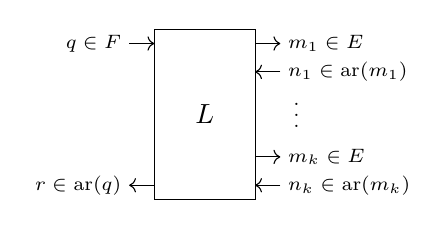
\begin{tikzpicture}[yscale=0.18,xscale=0.32]
      \draw (1,-1) rectangle (5,11) node[midway] {$L$};
      \scriptsize
      \draw[->] (0,10) node[left] {$q \in F$} -- (1,10);
        \draw[->] (5,10) -- (6,10) node[right] {$m_1 \in E$};
        \draw[->] (6,8) node[right] {$n_1 \in \kw{ar}(m_1)$} -- (5,8) ;
        \node[right] at (6,5.5) {$\:\vdots$};
        \draw[->] (5,2) -- (6,2) node[right] {$m_k \in E$};
        \draw[->] (6,0) node[right] {$n_k \in \kw{ar}(m_k)$} -- (5,0);
      \draw[->] (1,0) -- (0,0) node[left] {$r \in \kw{ar}(q)$};
    \end{tikzpicture}
  \end{column}
  \end{columns}

  \pause \vfill
  \begin{example}[Our top-level specification]
    The strategy
    $\Gamma_\kw{hello} : \mathcal{S} \twoheadrightarrow \mathcal{P}$
    contains the play:
    \[
      \Gamma_\kw{hello} \: \ni \: \kw{run} \cdot
      \underline{\kw{write}_1[\texttt{"hello, world!\textbackslash{}n"}]} \cdot
      14 \cdot
      \underline{0}
    \]
  \end{example}

  \pause \vfill
  Strategies feature a simple ordering $\le$ (``is refined by'').
\end{frame}

\begin{frame}{Layered Composition of Strategies}
  The stragies $L_1 : F \twoheadrightarrow G$ and
  $L_2 : E \twoheadrightarrow F$ can be composed to obtain:
  \[
     L_1 \odot L_2 : E \twoheadrightarrow G
  \]
  \pause
  This is done by letting them interact over $F$
  in the following way:
  \[
    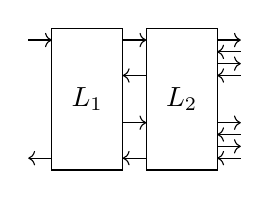
\begin{tikzpicture}[yscale=0.15,xscale=0.30]
      \draw (1,-1) rectangle (4,11) node[midway] {$L_1$};
      \draw (5,-1) rectangle (8,11) node[midway] {$L_2$};
      %\draw (5,-1) rectangle (8,4) node[midway] {$L_2$};
      \draw[->] (0,10) -- (1,10);
        \draw[->] (4,10) -- (5,10);
          \draw[->] (8,10) -- (9,10);
          \draw[->] (9,9) -- (8,9);
          \draw[->] (8,8) -- (9,8);
          \draw[->] (9,7) -- (8,7);
        \draw[->] (5,7) -- (4,7);
        \draw[->] (4,3) -- (5,3);
          \draw[->] (8,3) -- (9,3);
          \draw[->] (9,2) -- (8,2);
          \draw[->] (8,1) -- (9,1);
          \draw[->] (9,0) -- (8,0);
        \draw[->] (5,0) -- (4,0);
      \draw[->] (1,0) -- (0,0);
    \end{tikzpicture}
  \]

  \pause
  \begin{example}[Assembly linking]
    %To let $\kw{secret.s}$ call into $\kw{rot13.s}$ we can compute:
    %\[ \kw{Asm}(\kw{secret.s}) \odot \kw{Asm}(\kw{rot13.s}) \]
    A key ingredient in our example is
    the assembly linking theorem:
    \[ \ell \::\:
       \kw{Asm}(\kw{secret.s}) \odot \kw{Asm}(\kw{rot13.s}) \:\le\:
       \kw{Asm}(\kw{secret.s} + \kw{rot13.s}) \]
    The two strategies synchronize over $\kw{rot13()}$ calls,
    which become hidden internal calls.
  \end{example}
\end{frame}

\begin{frame}[fragile]{Layered Composition of Refinement Squares}
  Refinement is compatible with composition
  in the expected way:
  \[
    \begin{prooftree}
      \hypo{\only<3->{\phi:} L_1
         \le\only<6->{_{\mathbf{S} \twoheadrightarrow \mathbf{T}}} L_1'}
      \hypo{\only<3->{\psi:} L_2
         \le\only<6->{_{\mathbf{R} \twoheadrightarrow \mathbf{S}}} L_2'}
      \infer2{\only<4->{\phi \odot \psi \: : \: }
	L_1 \odot L_2 \:
        \le\only<6->{_{\mathbf{R} \twoheadrightarrow \mathbf{T}}}
        \: L_1' \odot L_2'}
    \end{prooftree}
  \]

  \pause
  This can be depicted as:

  \[
    \rule[-4em]{0pt}{8em}
    \begin{tikzcd}[sep=small]
       E \only<-3,5-6>{\ar[rr,"L_2",twoheadrightarrow]}
         \only<4,7>{\ar[rrrr,"L_1 \odot L_2",twoheadrightarrow]}
         \only<-5>{\ar[dd,equal]}
         \only<6->{\ar[dd,leftrightarrow,"\mathbf{R}"']}
       &&
       \only<-3,5-6>{%
       F \ar[rr,"L_1",twoheadrightarrow]
         \only<-5>{\ar[dd,equal]}
         \only<6->{\ar[dd,leftrightarrow,"\mathbf{S}"]}
       }%
       &&
       G \only<-5>{\ar[dd,equal]}
         \only<6->{\ar[dd,leftrightarrow,"\mathbf{T}"]}
       \\
       & \only<-2>{\le} \only<3,5-6>{\phi} &
         \only<4,7>{\phi \odot \psi} &
         \only<-2>{\le} \only<3,5-6>{\psi} &
       \\
       E\only<6->{'}
          \only<-3,5-6>{\ar[rr,"L_2'"',twoheadrightarrow]}
          \only<4,7>{\ar[rrrr, "L_1' \odot L_2'"', twoheadrightarrow]}
       &&
       \only<-3,5-6>{
         F\only<6->{'} \ar[rr,"L_1'"',twoheadrightarrow]
       }
       &&
       G\only<6->{'} \\
    \end{tikzcd}
  \]
\end{frame}

\begin{frame}[fragile]{Vertical Composition}
  \begin{columns}
    \begin{column}{0.6\textwidth}
      As expected, refinement $\le$ is transitive:
      \[
        \begin{prooftree}
          \hypo{\phi : L_1
            \le\only<4->{_{\mathbf{R} \twoheadrightarrow \mathbf{S}}}
            L_2}
          \hypo{\psi : L_2
            \le\only<4->{_{\mathbf{R'} \twoheadrightarrow \mathbf{S'}}} L_3}
          \infer2{\phi \vcomp \psi :
            L_1
              \le\only<4->{_{\mathbf{R} \vcomp \mathbf{R'} \twoheadrightarrow
                \mathbf{S} \vcomp \mathbf{S'}}}
            L_3}
        \end{prooftree}
      \]

      \uncover<3->{%
        This generalizes to refinement squares \\
        where the \emph{vertical composition} principle $\vcomp$ \\
        acts on refinement conventions as well.
      }

      \vspace{1em}
      \uncover<6->{%
        \begin{example}[Correctness and compilation]
          A correctness property
          $\Gamma_\kw{foo} \le_{\varnothing \twoheadrightarrow \mathbf{R}}
           \kw{Clight}(\kw{foo.c})$
          can be combined with the compiler correctness property
          \[ \kw{Clight}(\kw{foo.c})
           \le_{\mathbb{C} \twoheadrightarrow
                \mathbb{C}} \kw{Asm}(\kw{foo.s}) \]
          to obtain an end-to-end result.
        \end{example}
      }
    \end{column}
    \begin{column}{0.3\textwidth}
      \[
        \begin{tikzcd}[sep=small]
          E\only<4->{_1} \ar[rr, "L_1", twoheadrightarrow]
              \only<1>{\ar[dd, equal]}
              \only<2-3>{\ar[dddd,equal]}
              \only<4>{\ar[dd, "\mathbf{R}"', leftrightarrow]}
              \only<5->{\ar[dddd, "\mathbf{R} \vcomp \mathbf{R}'"', leftrightarrow]}
              &&
          F\only<4->{_1}
              \only<1>{\ar[dd, equal]}
              \only<2-3>{\ar[dddd,equal]}
              \only<4>{\ar[dd, "\mathbf{S}", leftrightarrow]}
              \only<5->{\ar[dddd, "\mathbf{S} \vcomp \mathbf{S}'", leftrightarrow]}
          \\
          & \only<2-3,5->{\color{white}} \phi &
          \\
          \only<1,4>{
          E\only<4->{_2} \ar[rr, "L_2", twoheadrightarrow]
            \only<-3>{\ar[dd, equal]}
            \only<4->{\ar[dd, "\mathbf{R}'"', leftrightarrow]}
          }
          &
          \only<1,4>{\color{white}}
          \!\!\!\! \phi \vcomp \psi \!\!\!\!
          &
          \only<1,4>{
          F\only<4->{_2}
            \only<-3>{\ar[dd, equal]}
            \only<4->{\ar[dd, "\mathbf{S}'", leftrightarrow]}
          }
          \\
          & \only<2-3,5->{\color{white}} \psi &
          \\
          E\only<4->{_3} \ar[rr, "L_3", twoheadrightarrow]
              &&
          F\only<4->{_3}
        \end{tikzcd}
      \]
    \end{column}
  \end{columns}
\end{frame}

\begin{frame}[fragile]{Flat composition}
  The operations of two signatures can be combined into one.

  \pause
  This \textbf{flat composition} operation $\oplus$ acts
  on the other objects as well:
  \pause
  \[
    \begin{tikzcd}[sep=tiny]
      E_1 \ar[rrrrrr, twoheadrightarrow, "L_1"]
          \ar[dddddd, leftrightarrow, "\mathbf{R_1}"']
          \ar[rd, dotted, dash] & & &&&&
      F_1 \ar[dddddd, leftrightarrow, "\mathbf{S_1}"]
          \ar[rd, dotted, dash]  & & \\
      & \oplus \ar[rd, dotted, dash] & &&&&
      & \oplus \ar[rd, dotted, dash] & \\
      & & E_2 \ar[rrrrrr, twoheadrightarrow, "L_2"]
              \ar[dddddd, leftrightarrow, "\mathbf{R}_2"'] &&&&
      & & F_2 \ar[dddddd, leftrightarrow, "\mathbf{S}_2"] \\
      \\ &&&& \color{white} \Big| XX \\ \\
      E_1' \ar[rrrrrr, twoheadrightarrow, "L_1'"']
           \ar[rd, dotted, dash] & & &&&&
      F_1' \ar[rd, dotted, dash] & & \\
      & \oplus \ar[rd, dotted, dash] & &&&&
      & \oplus \ar[rd, dotted, dash] & \\
      & & E_2' \ar[rrrrrr, twoheadrightarrow, "L_2'"'] &&&&
      & & F_2'
    \end{tikzcd}
    \qquad
    \begin{array}{c}
    \begin{prooftree}
      \hypo{L_1 : E_1 \twoheadrightarrow F_1}
      \hypo{L_2 : E_2 \twoheadrightarrow F_2}
      \infer2{
        L_1 \oplus L_2 : E_1 \oplus E_2 \twoheadrightarrow F_1 \oplus F_2}
    \end{prooftree}
    \\[2em] \pause
    \begin{prooftree}
      \hypo{\mathbf{R} : E_1 \leftrightarrow F_1}
      \hypo{\mathbf{S} : E_2 \leftrightarrow F_2}
      \infer2{
        \mathbf{R} \oplus \mathbf{S} : E_1 \oplus E_2 \leftrightarrow F_1 \oplus F_2
      }
    \end{prooftree}
    \\[2em] \pause
    \begin{prooftree}
      \hypo{\phi: L_1 \le_{\mathbf{R}_1 \twoheadrightarrow \mathbf{S}_1} L_1'}
      \hypo{\psi: L_2 \le_{\mathbf{R}_2 \twoheadrightarrow \mathbf{S}_2} L_2'}
      \infer2{\phi \oplus \psi :
	L_1 \oplus L_2
        \le_{\mathbf{R}_1 \oplus \mathbf{R}_2 \twoheadrightarrow
             \mathbf{S}_1 \oplus \mathbf{S}_2}
	L_1' \oplus L_2'}
    \end{prooftree}
    \end{array}
  \]
\end{frame}

\begin{frame}[fragile]{Flat composition}
  \begin{example}[Pipe operator]
    The system call interface $\mathcal{S}$
    can be decomposed by file descriptor:
    \[
      \mathcal{S} \cong \mathcal{F} \oplus \mathcal{F}
    \]
    Given two commands $P, Q : \mathcal{S} \twoheadrightarrow \mathcal{P}$
    we can define:
\[
  P \mathbin| Q \: := \:
    \kw{seq} \odot (P \oplus Q)
         \odot (\mathcal{F} \oplus (\Delta \odot \kw{fifo}) \oplus \mathcal{F})
\]
  [Add a figure and explain here]
  \end{example}
\end{frame}

\section{Managing State}

\begin{frame}{Motivation}
Our history-based strategy and refinement convention models \\
support hidden state, but this is not always what we want.

\vfill \pause
Ideally, we would like our refinement algebra to support state which is:
\begin{itemize}
  \item Visible locally, but hidden when we work on the next scale;
  \item Abstract at a high level of abstraction, more concrete as we implement;
  \item Hidden in specifications, but realized using low-level explicit memory.
\end{itemize}

\vfill \pause
Do deal with state in a flexible manner,
we introduce a \textbf{spatial composition} operator $\mathbin@$, \\
then leverage our refinement algebra to introduce
useful state management primitives.
\end{frame}

\begin{frame}{Spatial Composition}
The spatial composition operation $E \mathbin@ U$ annotates
every question and answer \\ with a state component taken in the set $U$:
\[
  E \mathbin@ U := \{ q @ u \mid q \in E, \, u \in U \}
  \qquad
  \kw{ar}_{E \mathbin@ U}(q @ u) := \kw{ar}_E(q) \times U
\]
Like $\oplus$, this operation acts coherently on all objects:
\[
  X
\]
\end{frame}

\begin{frame}{Manipulating state components}
To act on state components,
we use a kind of \textbf{stateful lenses}
$f : U \lensarrow V$ \\
which can be spatially composed with strategies:
\[
  \begin{prooftree}
    \hypo{L : E \twoheadrightarrow F}
    \hypo{f : U \lensarrow V}
    \infer2{L \mathbin@ f : E \mathbin@ U \twoheadrightarrow F \mathbin@ V}
  \end{prooftree}
\]

\pause
Similarly, relations between sets can be promoted to \\
and composed with refinement conventions: \\
\[
  \begin{prooftree}
    \hypo{\mathbf{R} : E \leftrightarrow F}
    \hypo{S \subseteq U \times V}
    \infer2{\mathbf{R} \mathbin@ S : E \mathbin@ U \twoheadrightarrow F \mathbin@ V}
  \end{prooftree}
\]

\pause
We also define refinement squares between lenses and they compose as expected.
\end{frame}

\begin{frame}[fragile]{Encapsulating state}
  State can be hidden using the encapsulation primitive:
  \[
    [u_0\rangle : U \leftrightarrows \mathbbm{1} \,,
  \]
  which maintains a hidden state of type $U$ with initial value $u_0 \in U$.

  \vfill \pause
  \begin{example}[Maybe the queue?]
  \end{example}
\end{frame}

\begin{frame}[fragile]{Representation Independence}
  When the initial states $u_0 \in U$ and $v_0 \in V$
  are related by $R \subseteq U \times V$,
  the refinement
  \[
    \begin{prooftree}
      \hypo{\phi_0 : u_0 \mathrel{R} v_0}
      \infer1{[\phi_0\rangle :
         [u_0\rangle \le_{R \twoheadrightarrow \mathbbm{1}}
         [v_0\rangle}
    \end{prooftree}
    \qquad \qquad
    \begin{tikzcd}[sep=tiny]
      U \ar[dd, "R"', leftrightarrow] \ar[rr, "{[u_0\rangle}"] &&
      \mathbbm{1} \ar[dd, equal] \\
      & {[ \phi_0 \rangle} & \\
      V \ar[rr, "{[v_0\rangle}"'] & & \mathbbm{1}
    \end{tikzcd}
  \]
  captures a form of \textbf{representation independence} property.

  \vfill \pause
  \begin{example}[continue previous example]
  \end{example}
\end{frame}

\begin{frame}[fragile]{Memory separation}
  Our state infrastructure can also incorporate
  \textbf{separation algebras} into our framework. \\
  A separation algebra $\bullet$ can be used as a relation
  $\mathsf{Y} \subseteq (\kw{mem} \times \kw{mem}) \times \kw{mem}$
  where
  \[
    (m_1, m_2) \mathrel{\mathsf{Y}} m \:\: :\Leftrightarrow \:\:
    m_1 \bullet m_2 = m
  \]
  The relation $\mathsf{Y}$ can then be used as a component in refinement conventions.

  \pause \vfill
  This allows us to formulate refinement-based \textbf{frame property};
  for example:
%  \[
%    \mathsf{FP}(p) \: : \:
%    \kw{Clight}(p) \mathbin@ \kw{mem}
%    \:
%    \le_{\mathcal{C} \mathbin@ \mathsf{Y} \twoheadrightarrow
%         \mathcal{C} \mathbin@ \mathsf{Y}}
%    \:
%    \kw{Clight}(p)
%  \]
  \[
    \begin{tikzcd}[row sep=tiny]
      \mathcal{C} \mathbin@ \kw{mem} \mathbin@ \kw{mem}
        \ar[rr, "\kw{Clight}(p) \mathbin@ \kw{mem}"]
        \ar[dd, "\mathcal{C} \mathbin@ \mathsf{Y}"] &&
      \mathcal{C} \mathbin@ \kw{mem} \mathbin@ \kw{mem}
        \ar[dd, "\mathcal{C} \mathbin@ \mathsf{Y}"]
      \\
      & \mathsf{FP}(p) &
      \\
      \mathcal{C} \mathbin@ \kw{mem}
        \ar[rr, "\kw{Clight}(p)"'] &&
      \mathcal{C} \mathbin@ \kw{mem}
    \end{tikzcd}
  \]
\end{frame}

\section{Conclusion}

\begin{frame}{Some Applications}
By combining these ingredients,
We were able to apply the framework in various ways:
\begin{itemize}
  \item Embed the language interfaces and semantics defined in CompCertO
  \item Formulate the compiler correctness theorem as a refinement square
  \item Define a new language ClightP with \emph{private} variables
  \item Construct a theory of certified abstraction layers
  \item Model the example from the introduction
\end{itemize}
\end{frame}

\begin{frame}{Conclusion}
  Points to take away:
  \begin{itemize}
    \item Advanced refinement frameworks could serve as coarse-grained glue
      in heterogeneous verification efforts
    %The potential role of refinement frameworks for coarse-grained reasoning
    \item Refinement conventions and alternating non-determinism in game semantics
    \item Thinking about compositionality geometrically
  \end{itemize}
\end{frame}

\end{document}
